\section{Additional figures}
\label{app:figures}

The four figures in this appendix show the baseline study in more detail.
They are computed from the released tables \texttt{data/evaluations.csv} and
\texttt{data/recommendations.csv} by the script
\texttt{analysis/19\_appendix\_figures.py}.

\begin{figure}[H]
\centering
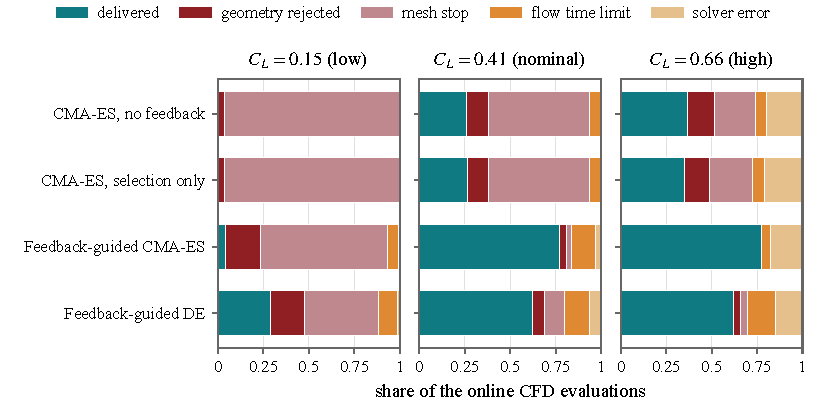
\includegraphics[width=\textwidth]{app_fig_yield_by_cell.pdf}
\caption{Outcomes of the online CFD evaluations of the four surrogate-assisted
baselines, by method and task. Each bar splits the 320 online evaluations of
one method on one task, 32 queries in each of 10 runs, by outcome. The outcome
is read from the reason codes in \texttt{data/evaluations.csv} and named as in
Table~\ref{tab:outcomes}. Delivered means CFD returned a complete score.
Geometry rejected means the mesh generator rejected the wing. Mesh stop means
the mesh generator stopped without a mesh. Flow time limit means a flow
condition reached its time limit. Solver error means the solver process
stopped with an error. An evaluation with both a time limit and a solver error
counts as a time limit. None of these evaluations falls in the other-errors
group of Table~\ref{tab:outcomes}, so that group is not shown.}
\label{fig:app-yield-by-cell}
\end{figure}

\begin{figure}[H]
\centering
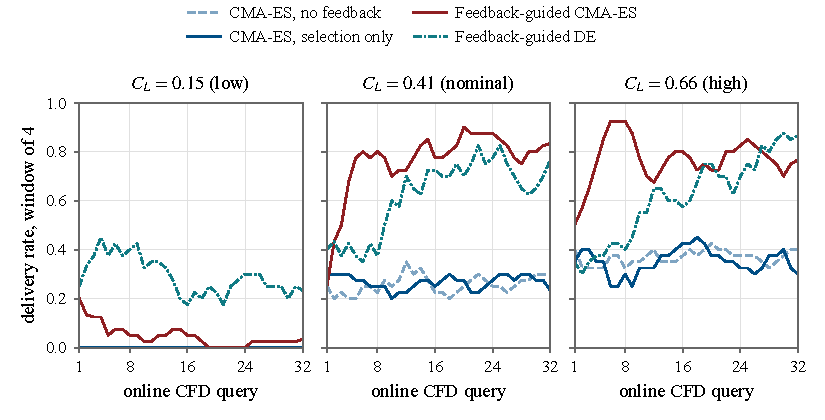
\includegraphics[width=\textwidth]{app_fig_online_yield_vs_index.pdf}
\caption{Online delivery rate along the run for the four surrogate-assisted
baselines, by task. For each method, task and query number from 1 to 32, the
delivery rate is the share of the 10 runs whose online evaluation at that
query returned a score, from the online rows of
\texttt{data/evaluations.csv}. Each curve is the moving average of these rates
over four neighboring queries, the query itself, the one before it and the two
after it, with fewer at the ends of the run.}
\label{fig:app-online-yield-vs-index}
\end{figure}

\begin{figure}[H]
\centering
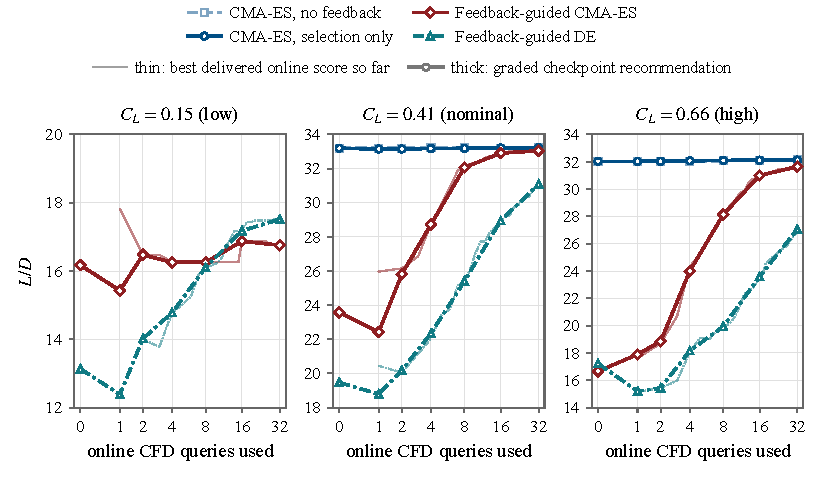
\includegraphics[width=\textwidth]{app_fig_discovery_vs_recommendation.pdf}
\caption{Best delivered online score against the score of the recommended
design, for the four surrogate-assisted baselines by task. The thin line is the
best $L/D$ a run had received from its online queries so far, averaged after
each query over the runs that had received at least one score by then, from
the online rows of \texttt{data/evaluations.csv}. The thick line is the mean
$L/D$ of the delivered recommendations at the checkpoints 0, 1, 2, 4, 8, 16 and
32 queries, from \texttt{data/recommendations.csv}. A checkpoint at which no
run's recommendation delivered is left out. Both lines use delivered scores
only. CMA-ES with no feedback and CMA-ES with selection only delivered nothing
at low load, so they do not appear in that panel. The horizontal axis is spaced
by the logarithm of the query count plus one.}
\label{fig:app-discovery-vs-recommendation}
\end{figure}

\begin{figure}[H]
\centering
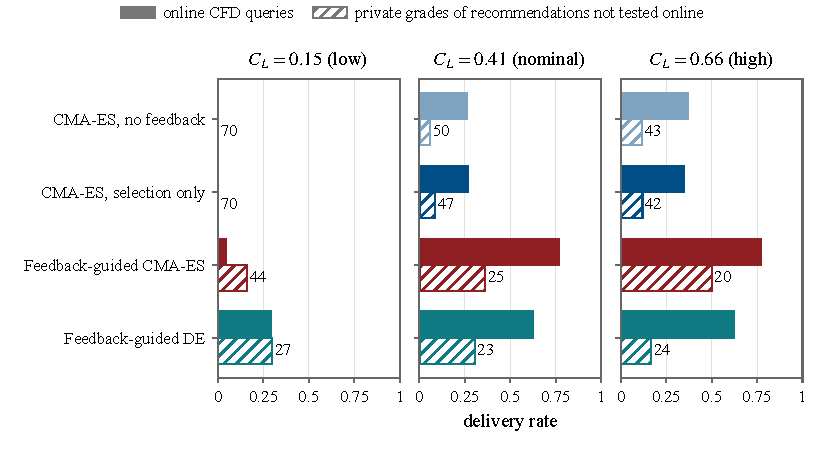
\includegraphics[width=\textwidth]{app_fig_fresh_hidden_vs_online_yield.pdf}
\caption{Delivery rate of the online CFD queries against the delivery rate of
the private grades, for the four surrogate-assisted baselines by task, from
\texttt{data/evaluations.csv}. The filled bar is the share of the 320 online
queries of one method on one task that returned a score. The hatched bar is
the share of its private grades that returned a score. A private grade is the
CFD evaluation of a recommended wing that the method had not queried online,
so the method never saw the result. The number next to each hatched bar is the
count of these private grades.}
\label{fig:app-fresh-hidden-vs-online-yield}
\end{figure}
